\begin{figure}
\centering

\begin{subfigure}[b]{0.25\columnwidth}
\centering
\cfbox{box-gray}{
\resizebox{!}{\textwidth}{
\tikzsetnextfilename{inter11}
\begin{tikzpicture}[
mynode/.style={draw, circle, very thick, inner sep=1pt, scale=1.3},
myline/.style={draw, very thick},
]
\pgfmathsetmacro{\n}{10};
\pgfmathsetmacro{\r}{2.5};

\node[mynode,draw=red] (1) at (0*360/\n + 90: \r cm) {$\xcolor{R}_1^1$};
\node[mynode,draw=red] (2) at (1*360/\n + 90: \r cm) {$\xcolor{R}_2^1$};
\node[mynode,draw=red] (3) at  (2*360/\n + 90: \r cm) {$\xcolor{R}_3^1$};
\node[mynode,draw=ForestGreen] (4) at  (3*360/\n + 90: \r cm) {$\xcolor{G}_1^1$};
\node[mynode,draw=ForestGreen] (5) at  (4*360/\n + 90: \r cm) {$\xcolor{G}_1^2$};
\node[mynode,draw=ForestGreen] (6) at  (5*360/\n + 90: \r cm) {$\xcolor{G}_2^1$};
\node[mynode,draw=ForestGreen] (7) at  (6*360/\n + 90: \r cm) {$\xcolor{G}_2^2$};
\node[mynode,draw=blue] (8) at  (7*360/\n + 90: \r cm) {$\xcolor{B}_1^1$};
\node[mynode,draw=blue] (9) at  (8*360/\n + 90: \r cm) {$\xcolor{B}_1^2$};
\node[mynode,draw=blue] (10) at  (9*360/\n + 90: \r cm) {$\xcolor{B}_1^3$};

\foreach \i in {1,...,\n}{
	\foreach \j in {\i,...,\n}{
    	\draw [myline,light-gray] (\i) -- (\j);
} }

\end{tikzpicture}
}
}
\caption{$K_{10}$.\label{fig:ch2:inter1_1}}
\end{subfigure}
%
% \hspace{0.02\textwidth}
%
\begin{subfigure}[b]{0.25\columnwidth}
\centering
\cfbox{box-gray}{
\resizebox{!}{\textwidth}{
\tikzsetnextfilename{inter12}
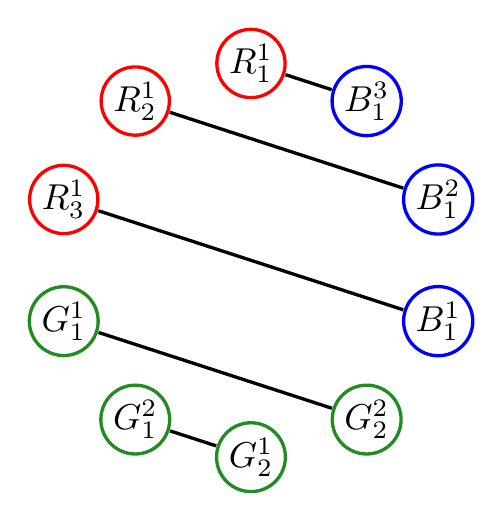
\begin{tikzpicture}[
mynode/.style={draw, circle, very thick, inner sep=1pt, scale=1.3},
myline/.style={draw, very thick},
]
\pgfmathsetmacro{\n}{10};
\pgfmathsetmacro{\r}{2.5};

\node[mynode,draw=red] (1) at (0*360/\n + 90: \r cm) {$\xcolor{R}_1^1$};
\node[mynode,draw=red] (2) at (1*360/\n + 90: \r cm) {$\xcolor{R}_2^1$};
\node[mynode,draw=red] (3) at  (2*360/\n + 90: \r cm) {$\xcolor{R}_3^1$};
\node[mynode,draw=ForestGreen] (4) at  (3*360/\n + 90: \r cm) {$\xcolor{G}_1^1$};
\node[mynode,draw=ForestGreen] (5) at  (4*360/\n + 90: \r cm) {$\xcolor{G}_1^2$};
\node[mynode,draw=ForestGreen] (6) at  (5*360/\n + 90: \r cm) {$\xcolor{G}_2^1$};
\node[mynode,draw=ForestGreen] (7) at  (6*360/\n + 90: \r cm) {$\xcolor{G}_2^2$};
\node[mynode,draw=blue] (8) at  (7*360/\n + 90: \r cm) {$\xcolor{B}_1^1$};
\node[mynode,draw=blue] (9) at  (8*360/\n + 90: \r cm) {$\xcolor{B}_1^2$};
\node[mynode,draw=blue] (10) at  (9*360/\n + 90: \r cm) {$\xcolor{B}_1^3$};

\draw [myline] (10) -- (1);
\draw [myline] (9) -- (2);
\draw [myline] (8) -- (3);
\draw [myline] (7) -- (4);
\draw [myline] (6) -- (5);

\end{tikzpicture}
}
}
\caption{\mypm{}~1.\label{fig:ch2:inter1_2}}
\end{subfigure}
%
% \hspace{0.02\textwidth}
%
\begin{subfigure}[b]{0.25\columnwidth}
\centering
\cfbox{box-gray}{
\resizebox{!}{\textwidth}{
\tikzsetnextfilename{inter13}
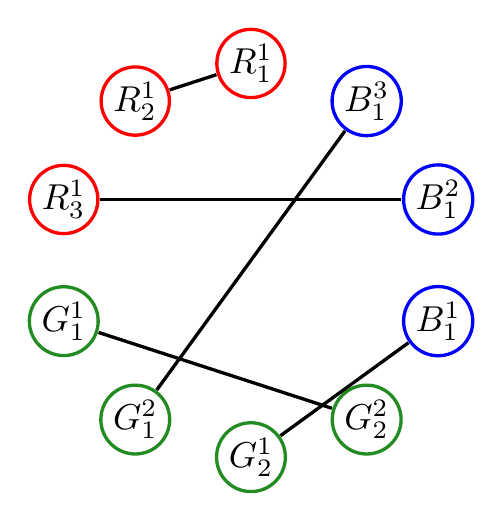
\begin{tikzpicture}[
mynode/.style={draw, circle, very thick, inner sep=1pt, scale=1.3},
myline/.style={draw, very thick},
]
\pgfmathsetmacro{\n}{10};
\pgfmathsetmacro{\r}{2.5};

\node[mynode,draw=red] (1) at (0*360/\n + 90: \r cm) {$\xcolor{R}_1^1$};
\node[mynode,draw=red] (2) at (1*360/\n + 90: \r cm) {$\xcolor{R}_2^1$};
\node[mynode,draw=red] (3) at  (2*360/\n + 90: \r cm) {$\xcolor{R}_3^1$};
\node[mynode,draw=ForestGreen] (4) at  (3*360/\n + 90: \r cm) {$\xcolor{G}_1^1$};
\node[mynode,draw=ForestGreen] (5) at  (4*360/\n + 90: \r cm) {$\xcolor{G}_1^2$};
\node[mynode,draw=ForestGreen] (6) at  (5*360/\n + 90: \r cm) {$\xcolor{G}_2^1$};
\node[mynode,draw=ForestGreen] (7) at  (6*360/\n + 90: \r cm) {$\xcolor{G}_2^2$};
\node[mynode,draw=blue] (8) at  (7*360/\n + 90: \r cm) {$\xcolor{B}_1^1$};
\node[mynode,draw=blue] (9) at  (8*360/\n + 90: \r cm) {$\xcolor{B}_1^2$};
\node[mynode,draw=blue] (10) at  (9*360/\n + 90: \r cm) {$\xcolor{B}_1^3$};

\draw [myline] (10) -- (5);
\draw [myline] (9) -- (3);
\draw [myline] (8) -- (6);
\draw [myline] (7) -- (4);
\draw [myline] (2) -- (1);

\end{tikzpicture}
}
}
\caption{\mypm{}~462.\label{fig:ch2:inter1_3}}
\end{subfigure}


\caption{Select interconnectivity graphs for \nameref{sec:ch2:example1}.\label{fig:ch2:inter1}}

\end{figure}

% \draw [] (10) -- (9);
% \draw [] (8) -- (2);
% \draw [] (7) -- (4);
% \draw [] (6) -- (5);
% \draw [] (3) -- (1);
% \caption{ 864 of 945 }